The following are comparisons between weirdospace images produced in the
experiment, through the Monte Carlo simulation, and by analytic means.
Noise has been added to some of the analytic images to ``get you in the
right mood''.
\newpage
\begin{figure}
	\begin{center}

		\makebox[0pt][r]{\parbox{2cm}{\raggedleft analytic}\hspace{0.25cm}}
		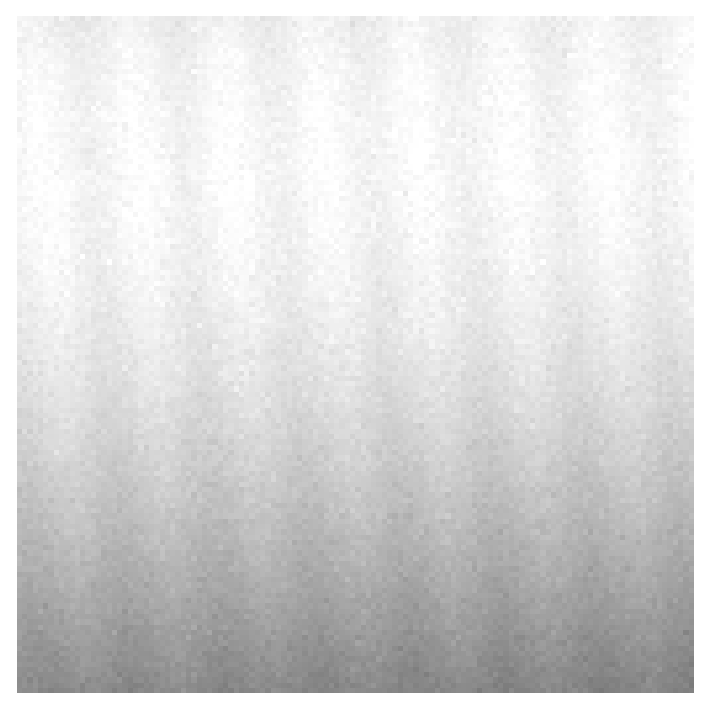
\includegraphics[width=3cm]{compare/allcmp/00180-theory.eps}
		\includegraphics[width=3cm]{compare/allcmp/blank.eps}
		\includegraphics[width=3cm]{compare/allcmp/blank.eps}
		\includegraphics[width=3cm]{compare/allcmp/blank.eps}\\

		\makebox[0pt][r]{\parbox{2cm}{\raggedleft Monte Carlo}\hspace{0.25cm}}
		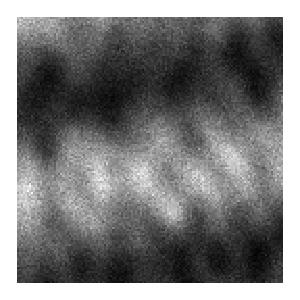
\includegraphics[width=3cm]{compare/allcmp/00180a-scatter.eps}
		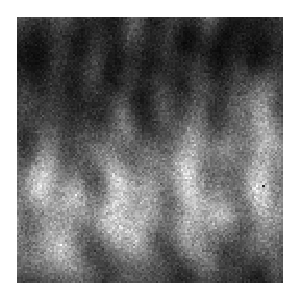
\includegraphics[width=3cm]{compare/allcmp/00180b-scatter.eps}
		\includegraphics[width=3cm]{compare/allcmp/blank.eps}
		\includegraphics[width=3cm]{compare/allcmp/blank.eps}\\
		\setcounter{subfigure}{0}

		\makebox[0pt][r]{\parbox{2cm}{\raggedleft experiment}\hspace{0.25cm}}
		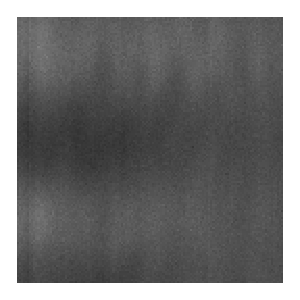
\includegraphics[width=3cm]{compare/allcmp/00180-01368_circ414.eps}
		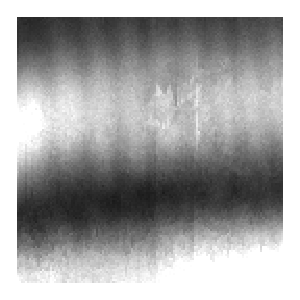
\includegraphics[width=3cm]{compare/allcmp/00180-01441_circ434.eps}
		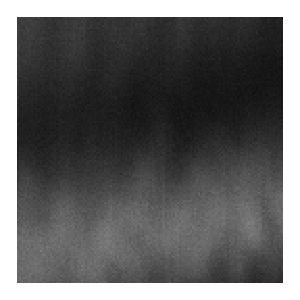
\includegraphics[width=3cm]{compare/allcmp/00180-01495_circ646.eps}
		\includegraphics[width=3cm]{compare/allcmp/00180-01576_circ559.eps}
	\end{center}
	\caption{Comparison of analytic, Monte Carlo, and experimental weirdospace
		in the vicinity of the \SI{180}{\degree} scattering direction.  The
		vertical features are secondary stripes produced by Equation~\ref{eqn:cbs}.}
	\label{fig:scat180degree}
\end{figure}

\begin{figure}
	\centering
	\begin{subfigure}[b]{0.32\textwidth}
		\centering
		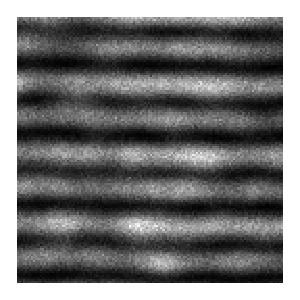
\includegraphics[width=3cm]{compare/allcmp/00002-scatter.eps}
		\caption{Monte Carlo}
	\end{subfigure}
	\begin{subfigure}[b]{0.32\textwidth}
		\centering
		\includegraphics[width=3cm]{compare/allcmp/00002-theory.eps}
		\caption{analytic}
	\end{subfigure}
	\caption{Comparison of Monte Carlo and analytic weirdospace in the
		vicinity of the \SI{0}{\degree} scattering direction.  The alternating
		intensity pattern is an interference between primary stripes and the two
		Type \Rmnum{3} events.}
	\label{fig:scat0degree}
\end{figure}

\begin{figure}
	\centering

	\makebox[0pt][r]{\parbox{2cm}{\raggedleft analytic}\hspace{0.25cm}}
	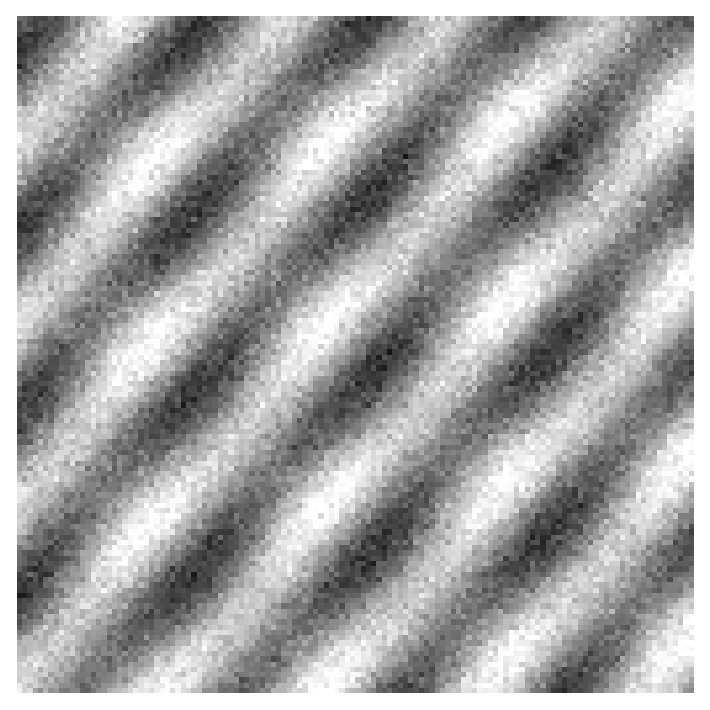
\includegraphics[width=3cm]{compare/allcmp/00085-theory.eps}
	\includegraphics[width=3cm]{compare/allcmp/blank.eps}\\

	\makebox[0pt][r]{\parbox{2cm}{\raggedleft Monte Carlo}\hspace{0.25cm}}
	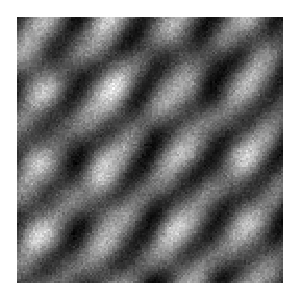
\includegraphics[width=3cm]{compare/allcmp/00085-scatter.eps}
	\includegraphics[width=3cm]{compare/allcmp/blank.eps}\\

	\makebox[0pt][r]{\parbox{2cm}{\raggedleft experiment}\hspace{0.25cm}}
	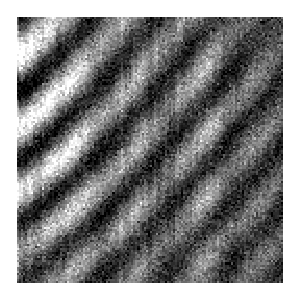
\includegraphics[width=3cm]{compare/allcmp/00085-00982_circ427}
	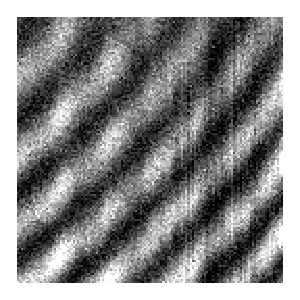
\includegraphics[width=3cm]{compare/allcmp/00085-01100_circ647}
	\caption{Comparison of analytic, Monte Carlo, and experimental weirdospace
		in the vicinity of the \SI{85}{\degree} scattering direction.  Note the
		distinct shape of the dark pockets predicted by the analytic and Monte
		Carlo simulations.  This shape is due to interference of the two Type
		\Rmnum{3} events.}
	\label{fig:scat85degree}
\end{figure}

\begin{figure}
	\centering

	\makebox[0pt][r]{\parbox{2cm}{\raggedleft analytic}\hspace{0.25cm}}
	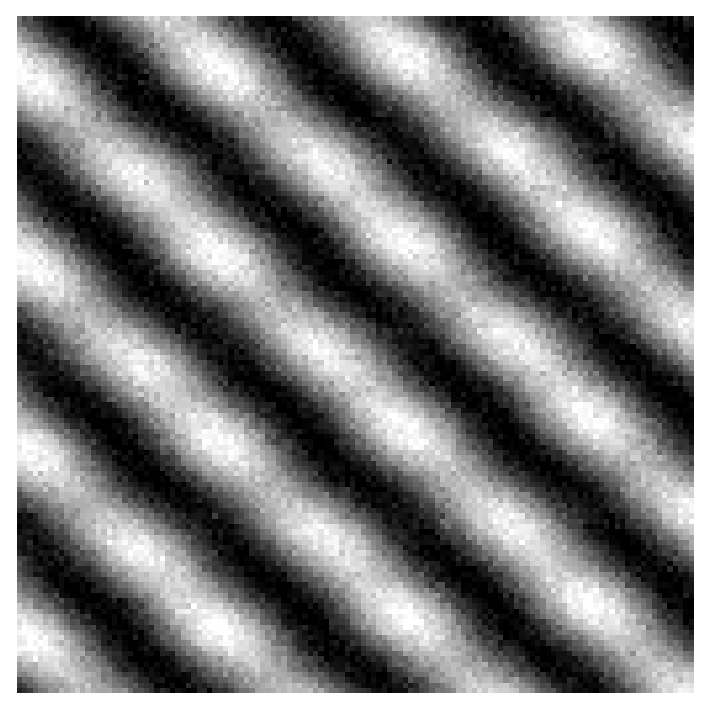
\includegraphics[width=3cm]{compare/allcmp/00270-theory.eps}
	\includegraphics[width=3cm]{compare/allcmp/blank.eps}\\

	\makebox[0pt][r]{\parbox{2cm}{\raggedleft Monte Carlo}\hspace{0.25cm}}
	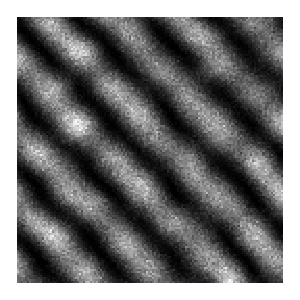
\includegraphics[width=3cm]{compare/allcmp/00270-scatter.eps}
	\includegraphics[width=3cm]{compare/allcmp/blank.eps}\\

	\makebox[0pt][r]{\parbox{2cm}{\raggedleft experiment}\hspace{0.25cm}}
	\includegraphics[width=3cm]{compare/allcmp/00270-00111_circ647.eps}
	
\includegraphics[width=3cm]{compare/allcmp/00270-00188_circ515.eps}
	\caption{Comparison of analytic, Monte Carlo, and experimental weirdospace
		in the vicinity of the \SI{270}{\degree} scattering direction.  Note the
		orientation of the secondary stripes and that they come in intensity groups
		of two.}
	\label{fig:scat270degree}
\end{figure}

\begin{figure}
	\begin{center}
		\addtolength{\subfigbottomskip}{-1cm}

		\makebox[0pt][r]{\parbox{3cm}{\raggedleft analytic, $E_\chi$ not included}\hspace{0.25cm}}
		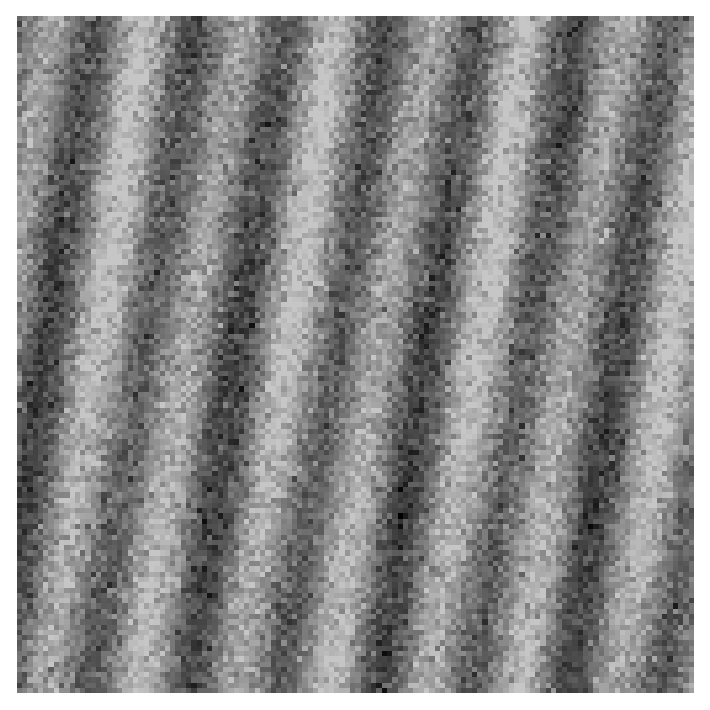
\includegraphics[width=3cm]{compare/allcmp/cbs-00016-theory.eps}
		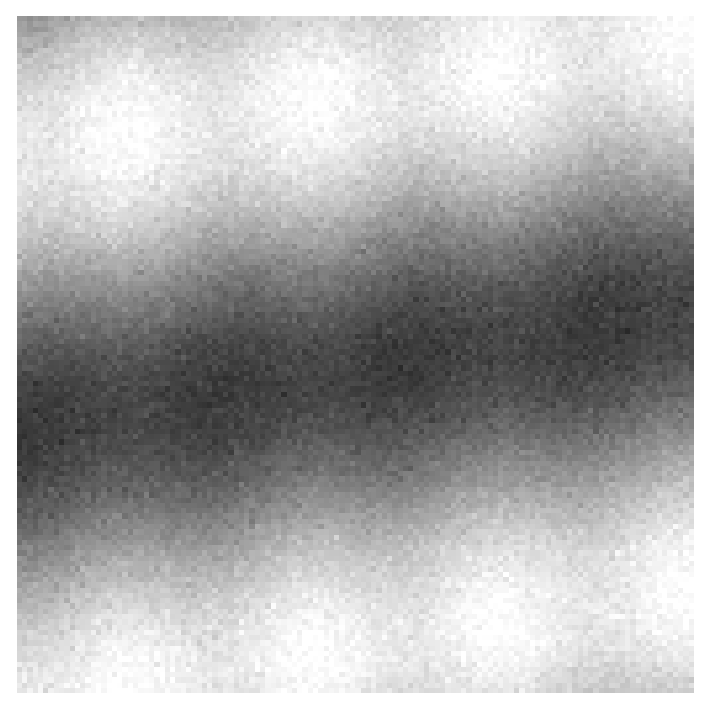
\includegraphics[width=3cm]{compare/allcmp/cbs-00160-theorya.eps}
		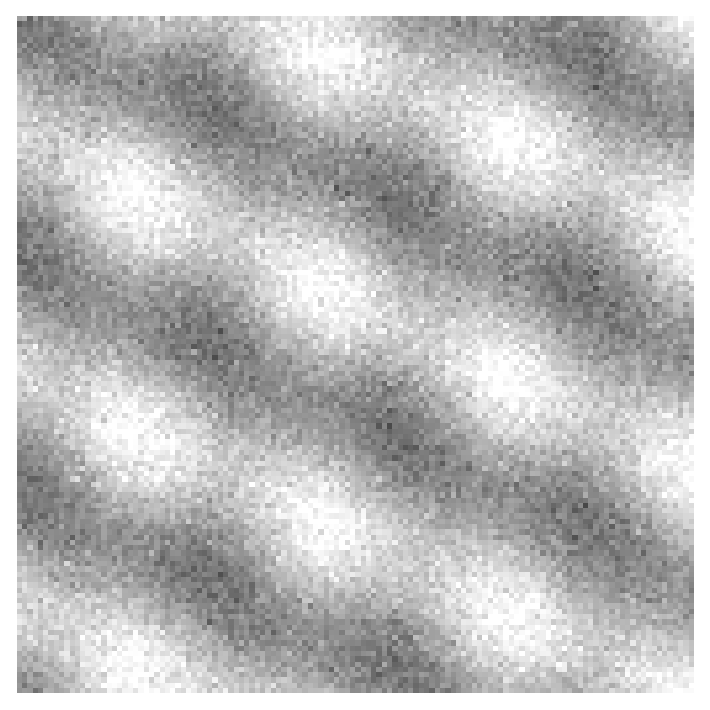
\includegraphics[width=3cm]{compare/allcmp/cbs-00233-theorya.eps}\\

		\makebox[0pt][r]{\parbox{3cm}{\raggedleft Monte Carlo, no time reverse paths.}\hspace{0.25cm}}
		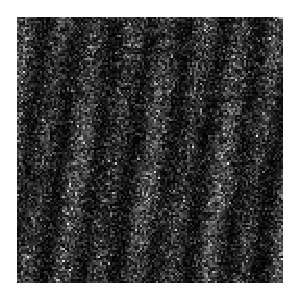
\includegraphics[width=3cm]{compare/allcmp/cbs-00016-scatter-notr.eps}
		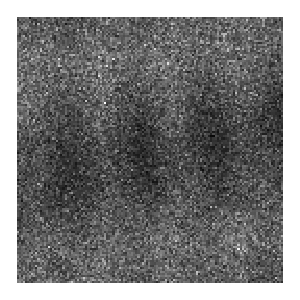
\includegraphics[width=3cm]{compare/allcmp/cbs-00160-scatter-notr.eps}
		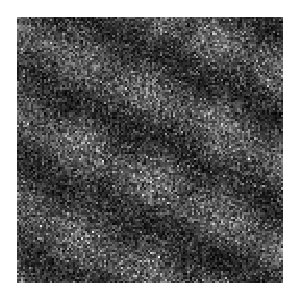
\includegraphics[width=3cm]{compare/allcmp/cbs-00233-scatter-notr.eps}\\

		\makebox[0pt][r]{\parbox{3cm}{\raggedleft analytic, $E_\chi$ included}\hspace{0.25cm}}
		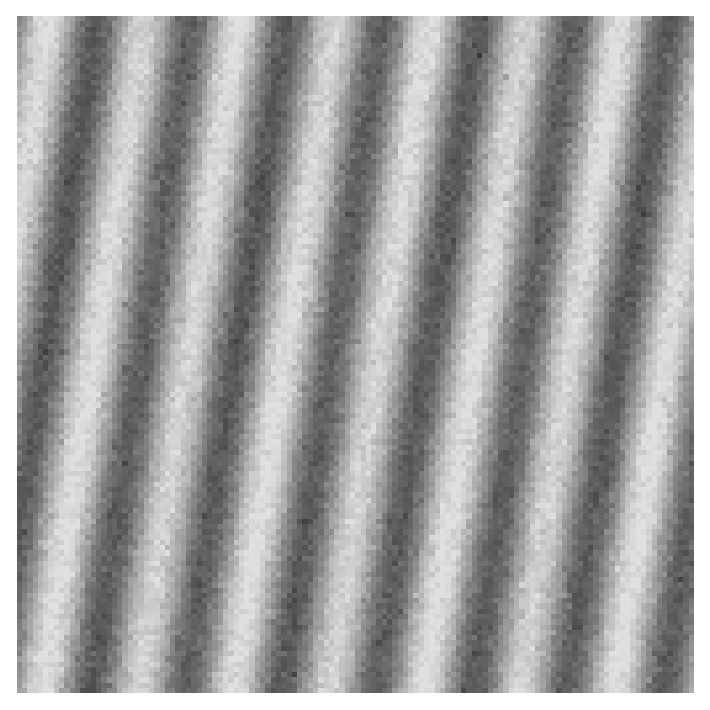
\includegraphics[width=3cm]{compare/allcmp/cbs-00016-theoryb.eps}
		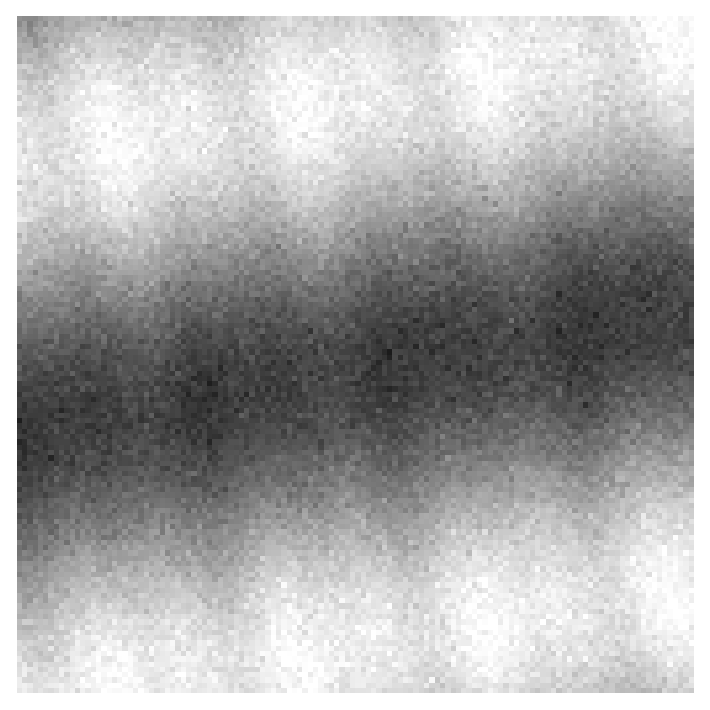
\includegraphics[width=3cm]{compare/allcmp/cbs-00160-theoryb.eps}
		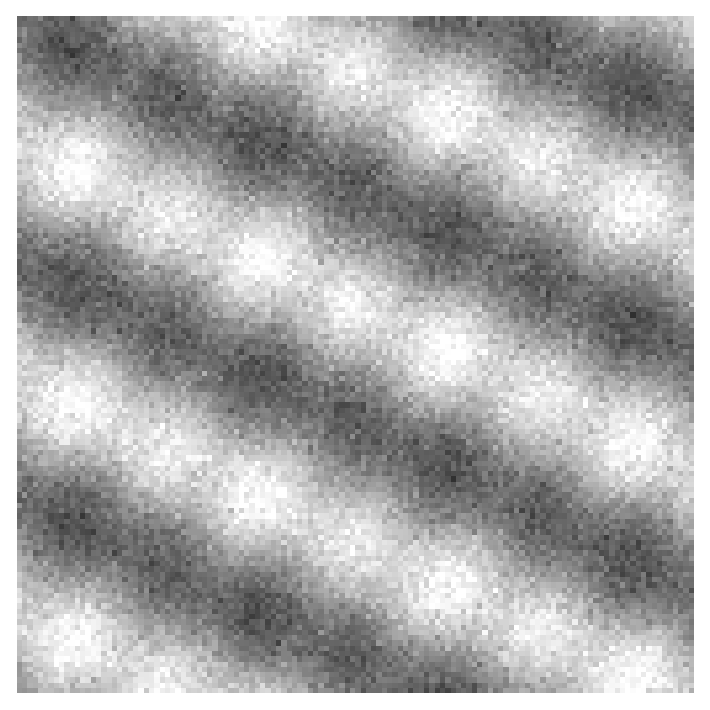
\includegraphics[width=3cm]{compare/allcmp/cbs-00233-theoryb.eps}\\

		\setcounter{subfigure}{0}
		\makebox[0pt][r]{\parbox{3cm}{\raggedleft Monte Carlo, time reverse paths included.}\hspace{0.25cm}}
		\begin{subfigure}[b]{0.32\textwidth}
			\centering
			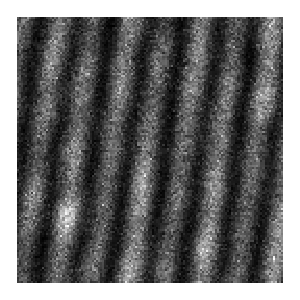
\includegraphics[width=3cm]{compare/allcmp/cbs-00016-scatter-withtr.eps}
			\caption{\SI{16}{\degree}}
		\end{subfigure}
		\begin{subfigure}[b]{0.32\textwidth}
			\centering
			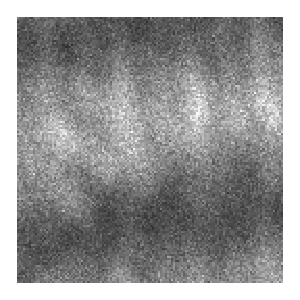
\includegraphics[width=3cm]{compare/allcmp/cbs-00160-scatter-withtr.eps}
			\caption{\SI{160}{\degree}}
		\end{subfigure}
		\begin{subfigure}[b]{0.32\textwidth}
			\centering
			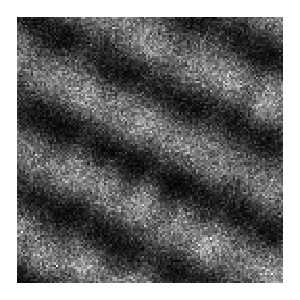
\includegraphics[width=3cm]{compare/allcmp/cbs-00233-scatter-withtr.eps}
			\caption{\SI{233}{\degree}}
		\end{subfigure}\\
	\end{center}
	\caption{Comparison of analytic and Monte Carlo simulations in the case
		where time reverse paths (Equation \ref{eqn:cbs}) have been removed from
		either.}
	\label{fig:rtr}
\end{figure}

\begin{figure}
	\centering
	\begin{subfigure}[b]{0.32\textwidth}
		\centering
		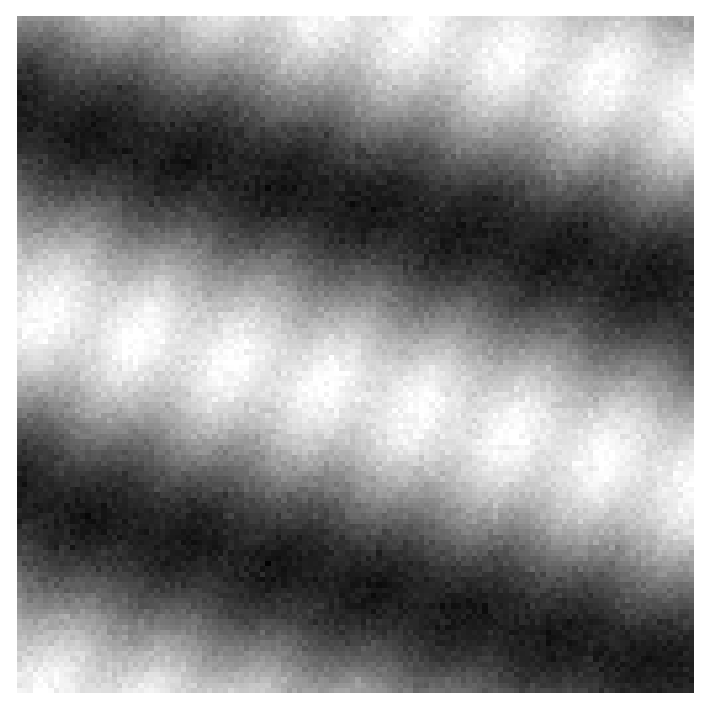
\includegraphics[width=3cm]{compare/allcmp/d1-theory.eps}
		\caption{analytic}
	\end{subfigure}
	\begin{subfigure}[b]{0.32\textwidth}
		\centering
		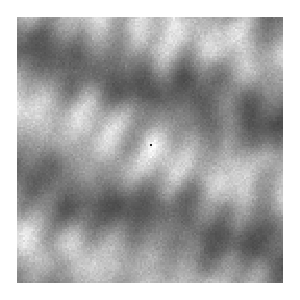
\includegraphics[width=3cm]{compare/allcmp/d1-00213-scatter.eps}
		\caption{Monte Carlo}
	\end{subfigure}
	\begin{subfigure}[b]{0.32\textwidth}
		\centering
		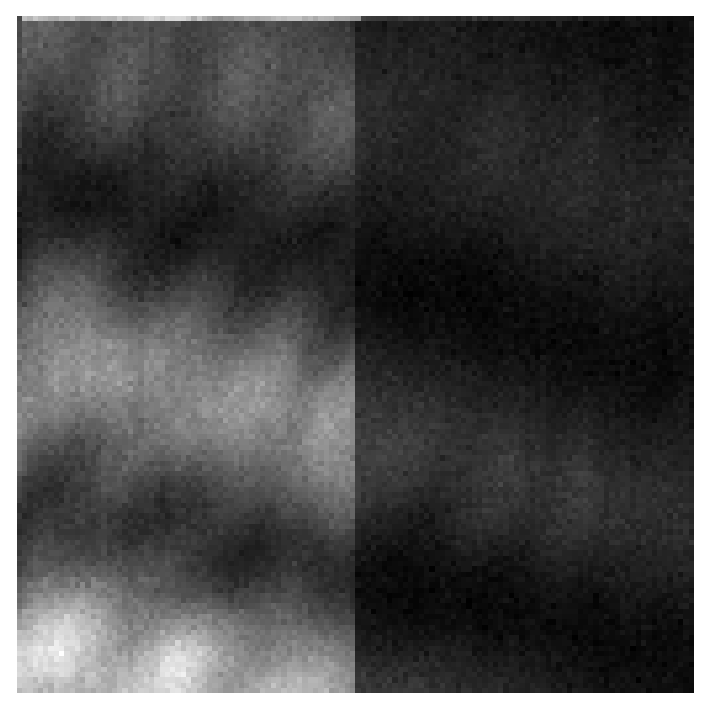
\includegraphics[width=3cm]{compare/allcmp/d1-experiment.eps}
		\caption{experiment}
	\end{subfigure}
	\caption{Comparison of analytic and experimental weirdospace for some angle
		around the ring.  Note the relationship between intensity maxima on each
		primary stripe and their ``hexagonal packing'' relationship.  Also, the way
		these maxima connects with another with a thin, curvy intensity.  This
		interference effect is from primary and secondary stripes.}
	\label{fig:hexagonalpacking1}
\end{figure}

\begin{figure}
	\centering
	\begin{subfigure}[b]{0.32\textwidth}
		\centering
		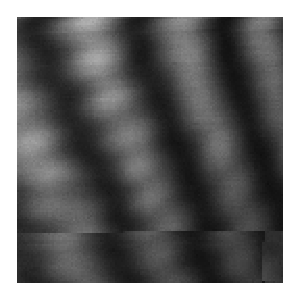
\includegraphics[width=3cm]{compare/allcmp/o1-00000_circ538.eps}
		\caption{scan538}
	\end{subfigure}
	\begin{subfigure}[b]{0.32\textwidth}
		\centering
		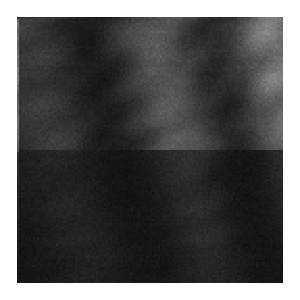
\includegraphics[width=3cm]{compare/allcmp/o1-01795_circ645.eps}
		\caption{scan645}
	\end{subfigure}
	\begin{subfigure}[b]{0.32\textwidth}
		\centering
		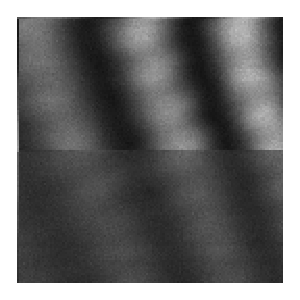
\includegraphics[width=3cm]{compare/allcmp/o1-01843_circ645.eps}
		\caption{scan645}
	\end{subfigure}
	\caption{Exhibition of some of the stripe features found in the
		experimental data.  Note the (alternating) relationship between intensity
		maxima on each primary stripe and their ``hexagonal packing''. This
		interference effect is from primary and secondary stripes.}
	\label{fig:hexagonalpacking2}
\end{figure}
